\section{Rechnungswesen mit SAP ERP Financials}
\subsection{Komponenten}
Das Ziel von ERP-Systemen (Enterprise Resource Planning \abk{ERP}{Enterprise Resource Planning}) ist die Erfassung aller wesentlichen betrieblichen Abläufe zur Planung, Dokumentation und Steuerung. Die ERP-Software der Firma SAP ist eine branchenübergreifende Standardlösung, die sich an unterschiedlichste Anforderungen verschiedener Unternehmen anpassen lässt (Customizing\abk{Customizing}{Softwareanpassung an betriebs- und branchenspezifische Vorgaben}). Die Anwendungen erlauben eine ganzheitliche Abwicklung von abteilungs- und\\bereichsübergreifenden Prozessen der organisatorischen Einheit. Die Struktur von SAP ERP orientiert sich an den klassischen betriebswirtschaftlichen Funktionen eines Unternehmens. Auf der obersten Ebene finden sich die funktionalen Sichten:
\begin{compactitem}
\item Finanzen
\item Personalwirtschaft
\item Beschaffung und Logistik
\item Produktion
\item Vertrieb
\end{compactitem}
Diese Struktur wird weiter in Komponenten, Unterkomponenten und Transaktionen aufgeteilt. Während die Firma SAP für diese Komponenten des bereits 1992 erschienenen SAP R/3 noch klare Modulbezeichnungen etabliert hat, verzichtet sie im heutigen Marketing der Weiterentwicklung SAP ERP darauf\footnote{Vgl. \cite{Klein2010}, S. 9 f.}\footnote{Vgl. \cite{Hefner2001}, S. 25}. Für eine exakte Einordnung im Themenkomplex, werden in dieser Arbeit auch die Modulbezeichnungen beigefügt.

SAP ERP Financials als Teil von SAP ERP ist die Anwendung für die Unternehmenssicht Finanzen, welche folgende Komponenten beinhaltet\footnote{Vgl. \cite{Hefner2001}, S. 27}:
\begin{compactitem}
\item Financial Accounting (Finanzwesen -- FI)
\item Management Accounting (Controlling -- CO)
\item Enterprise Controlling (Unternehmenscontrolling -- EC)
\item Treasury (TR)
\item Investment Management (IM)
\end{compactitem}
Diese Arbeit konzentriert sich auf das Rechnungswesen (FI, CO) mit SAP ERP Financials, welches in den Komponenten Financial Accounting (FI) und Management Accounting (CO) abgebildet und in den folgenden Kapiteln näher behandelt wird\footnote{Vgl. \cite{Patel2009}, S. 23}.

\subsection{Konzernstruktur}
\begin{figure}[htbp]
\begin{center}
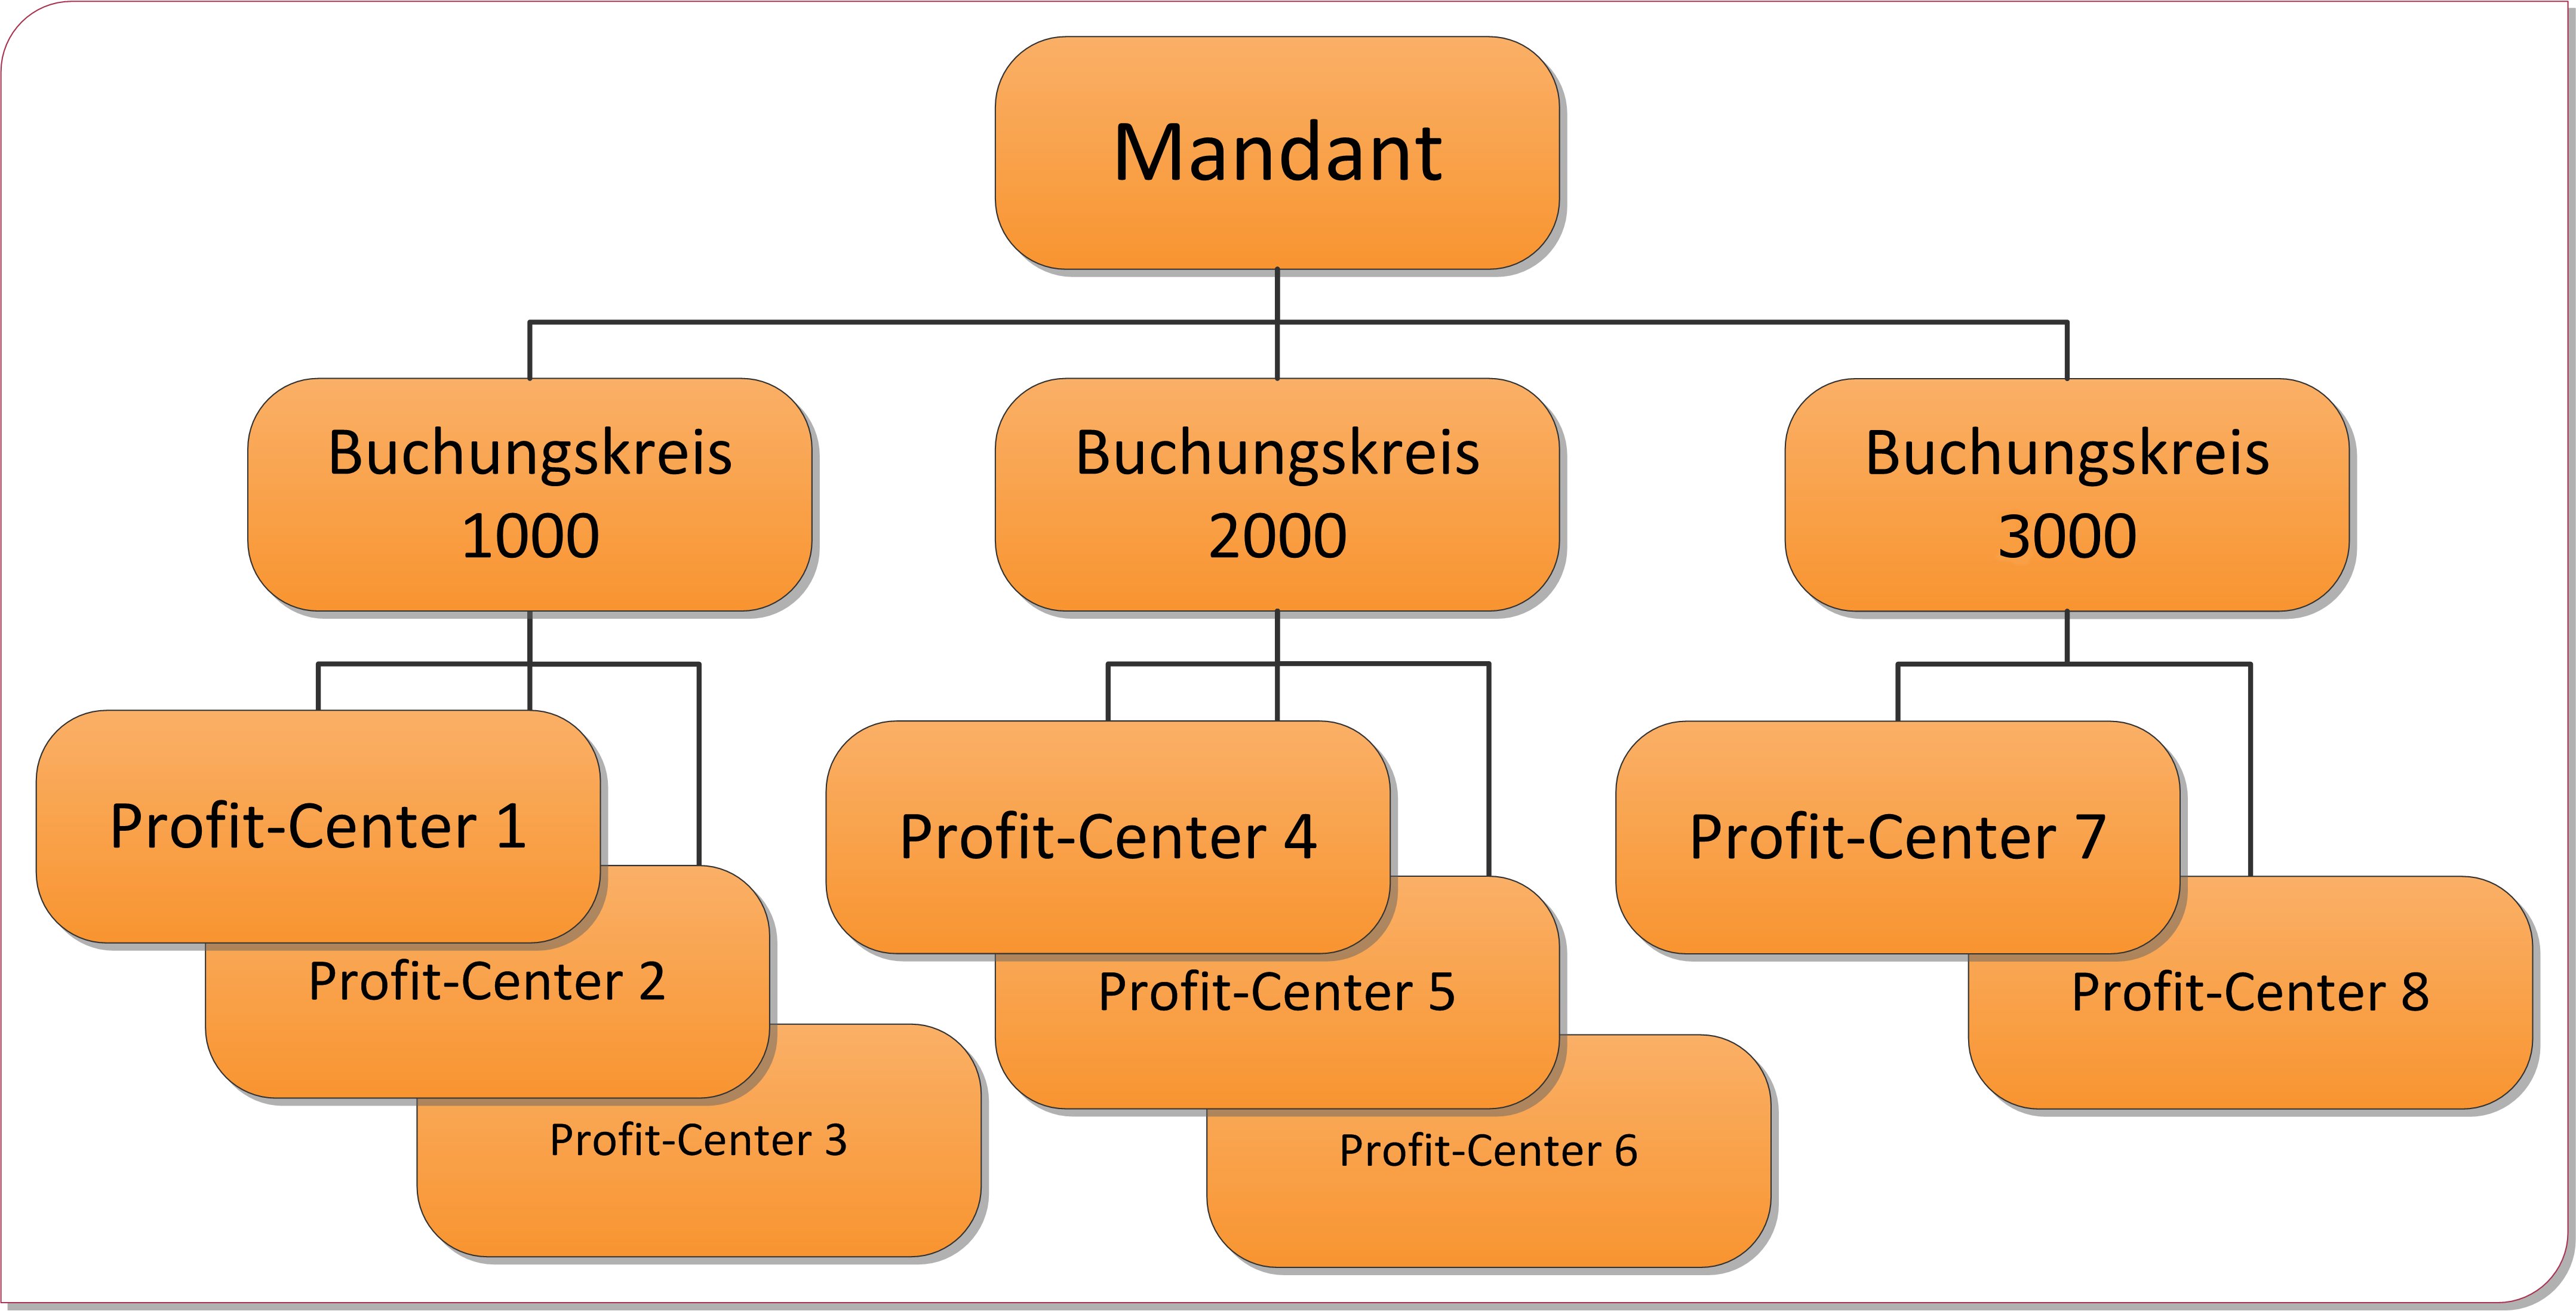
\includegraphics[width=0.9\textwidth]{Images/konzernStruktur.png}

   %{\footnotesize In Anlehnung an: \cite{Hefner2001}, S. 100}
   \caption[Konzernstruktur in SAP ERP Financials]{Konzernstruktur in SAP ERP Financials}\label{abb2}
\end{center}
\end{figure}\noindent
Bei der Einführung eines SAP ERP-Systems müssen die betrieblichen Organisationsstrukturen, die sich aus unterschiedlichen Gesellschaften und operativen Einheiten eines Konzerns zusammensetzt, in diesem abgebildet werden.
Jede Komponente des SAP ERP Systems hat ihre eigenen Organisationsstrukturen\footnote{Vgl. \cite{Klein2010}, S. 98}. Im Folgenden werden die Organisationseinheiten des internen und externen Rechnungswesens beschrieben. Abbildung~\ref{abb2} auf Seite \pageref{abb2} zeigt ein Beispiel einer Konzernstruktur im SAP Rechnungswesen.

Der Mandant stellt die oberste Konzernhierarchieebene dar und bildet ein Konzernunternehmen mit allen zugehörigen Gesellschaften ab, deren Ergebnisse in das Konzernergebnis einfließen. Gesellschaftsübergreifende Daten und Parameter werden auf Mandantenebene abgelegt.
%################## Kostenrechnungkreis?? #############
Die wichtigsten Organisationseinheiten innerhalb eines Mandanten sind die Buchungskreise. Unter einem Buchungskreis versteht man in SAP ERP Financials selbständig bilanzierende Einheiten der Finanzbuchhaltung. Jeder Buchungskreis erhält eine eigene Bilanz und GuV (Gewinn- und Verlustrechnung)\abk{GuV}{Gewinn- und Verlustrechnung}. Die Konzernabschlüsse werden ja Buchungskreis nach den geltenden gesetzlichen Anforderungen erstellt. Wenn die Unternehmung/Konzern nur aus einer Einheit zusammengesetzt sein sollte, wird in SAP ERP Financials mindestens ein Buchungskreis eingerichtet.

Die Organisationsebene Geschäftsbereich wird zu Auswertungszwecken eingesetzt. Er wird nicht mehr weiter entwickelt und diente als zusätzliche Möglichkeit, Konzernabschlüsse auf Grundlage zentraler operativer Bereiche (z. B. Produktlinien, Zweigstellen oder strategische Geschäftseinheiten) zu erstellen, welche jedoch nicht den Anforderungen externer Bilanzen und GuV entsprechen. In neueren Implementierungen wird für die Segmentberichterstattung auf andere Organisationseinheiten (z. B. Profit-Center oder Segmente) zurückgegriffen.

Profit-Center sind verwaltungsorientierte Konzernstrukturen (z. B. Bereiche oder Abteilungen). Profit-Center ermöglichen, anhand der Gegenüberstellung gebuchter Kosten und Erlöse, eigene interne Betriebsergebnisse und Abschlüsse.

Für einzelne Segmente, die durch klassifizierende Merkmale beschrieben werden (z. B. Artikelgruppe, Kundengruppe, Land, Vertriebsweg), kann ein Ergebnis ausgewiesen werden. Die Segmente werden deshalb Ergebnisobjekte genannt. Obwohl bei der Definition von Segmenten keine Einschränkungen gelten, werden sie in der Regel von Profit-Centern abgeleitet und dienen in allen Gesellschaften zu Berichtszwecken. 

Um die Betriebsaufwendungen der GuV im Umsatzkostenverfahren entsprechend betrieblicher Funktionen wie Finanzen, Personalwirtschaft, Beschaffung und Logistik, Produktion oder Vertrieb gruppiert auszuweisen, kann die Organisationseinheit Funktionsbereich verwendet werden.

In der Komponente Management Accounting (CO) ist die zentrale Organisationseinheit der Kostenrechnungskreis. Ein Kostenrechnungskreis wird für alle organisatorischen Einheiten vergeben, für die eine vollständige, in sich geschlossene Kostenrechnung durchgeführt werden soll\footnote{Vgl. \cite{Hefner2001}, S. 99 ff.}\footnote{Vgl. \cite{Friedl2008}, S. 29 ff.}\footnote{Vgl. \cite{Maassen2006}, S. 71 ff.}\footnote{Vgl. \cite{Patel2009}, S. 37 ff.}\footnote{Vgl. \cite{Padhi2011}, S. 16}\footnote{Vgl. \cite{SAPFI2001}, S. 18}.







\subsection{Financial Accounting (FI)} %FI
\subsubsection{General Ledger} %Hauptbuch FI-GL -- #### ERST GEGEN ENDE SCHREIBEN!! Das neue Hauptbuch in FI vereint Funktionen aus FI und CO
\subsubsection{Accounts receivable and payable} %Debitoren FI-AR %Kreditoren FI-AP
\subsubsection{Tax Accounting} %Steuern

\subsubsection{Bank Accounting} %Bankbuchhaltung FI-BL
\subsubsection{Asset Accounting} %Anlagenbuchhaltung FI-AA

\subsection{Management Accounting (CO)} %CO
Die Komponente Management Accounting (Controlling -- CO) bildet die, in Kapitel \ref{ssec:internesRechnungswesen} internes Rechnungswesen auf Seite \pageref{ssec:internesRechnungswesen}, beschriebenen Funktionen in SAP ERP Financials ab und gliedert sich in die drei Unterkomponenten Overhead Cost Controlling (CO-OM), Product Cost Accounting (CO-PC) und Profitability Analysis (CO-PA). Abbildung \ref{abb3} auf Seite \pageref{abb3} zeigt die vollständig in der Finanzbuchhaltung und Kostenrechnung integrierten Komponenten. 
\begin{figure}[htbp]
\begin{center}
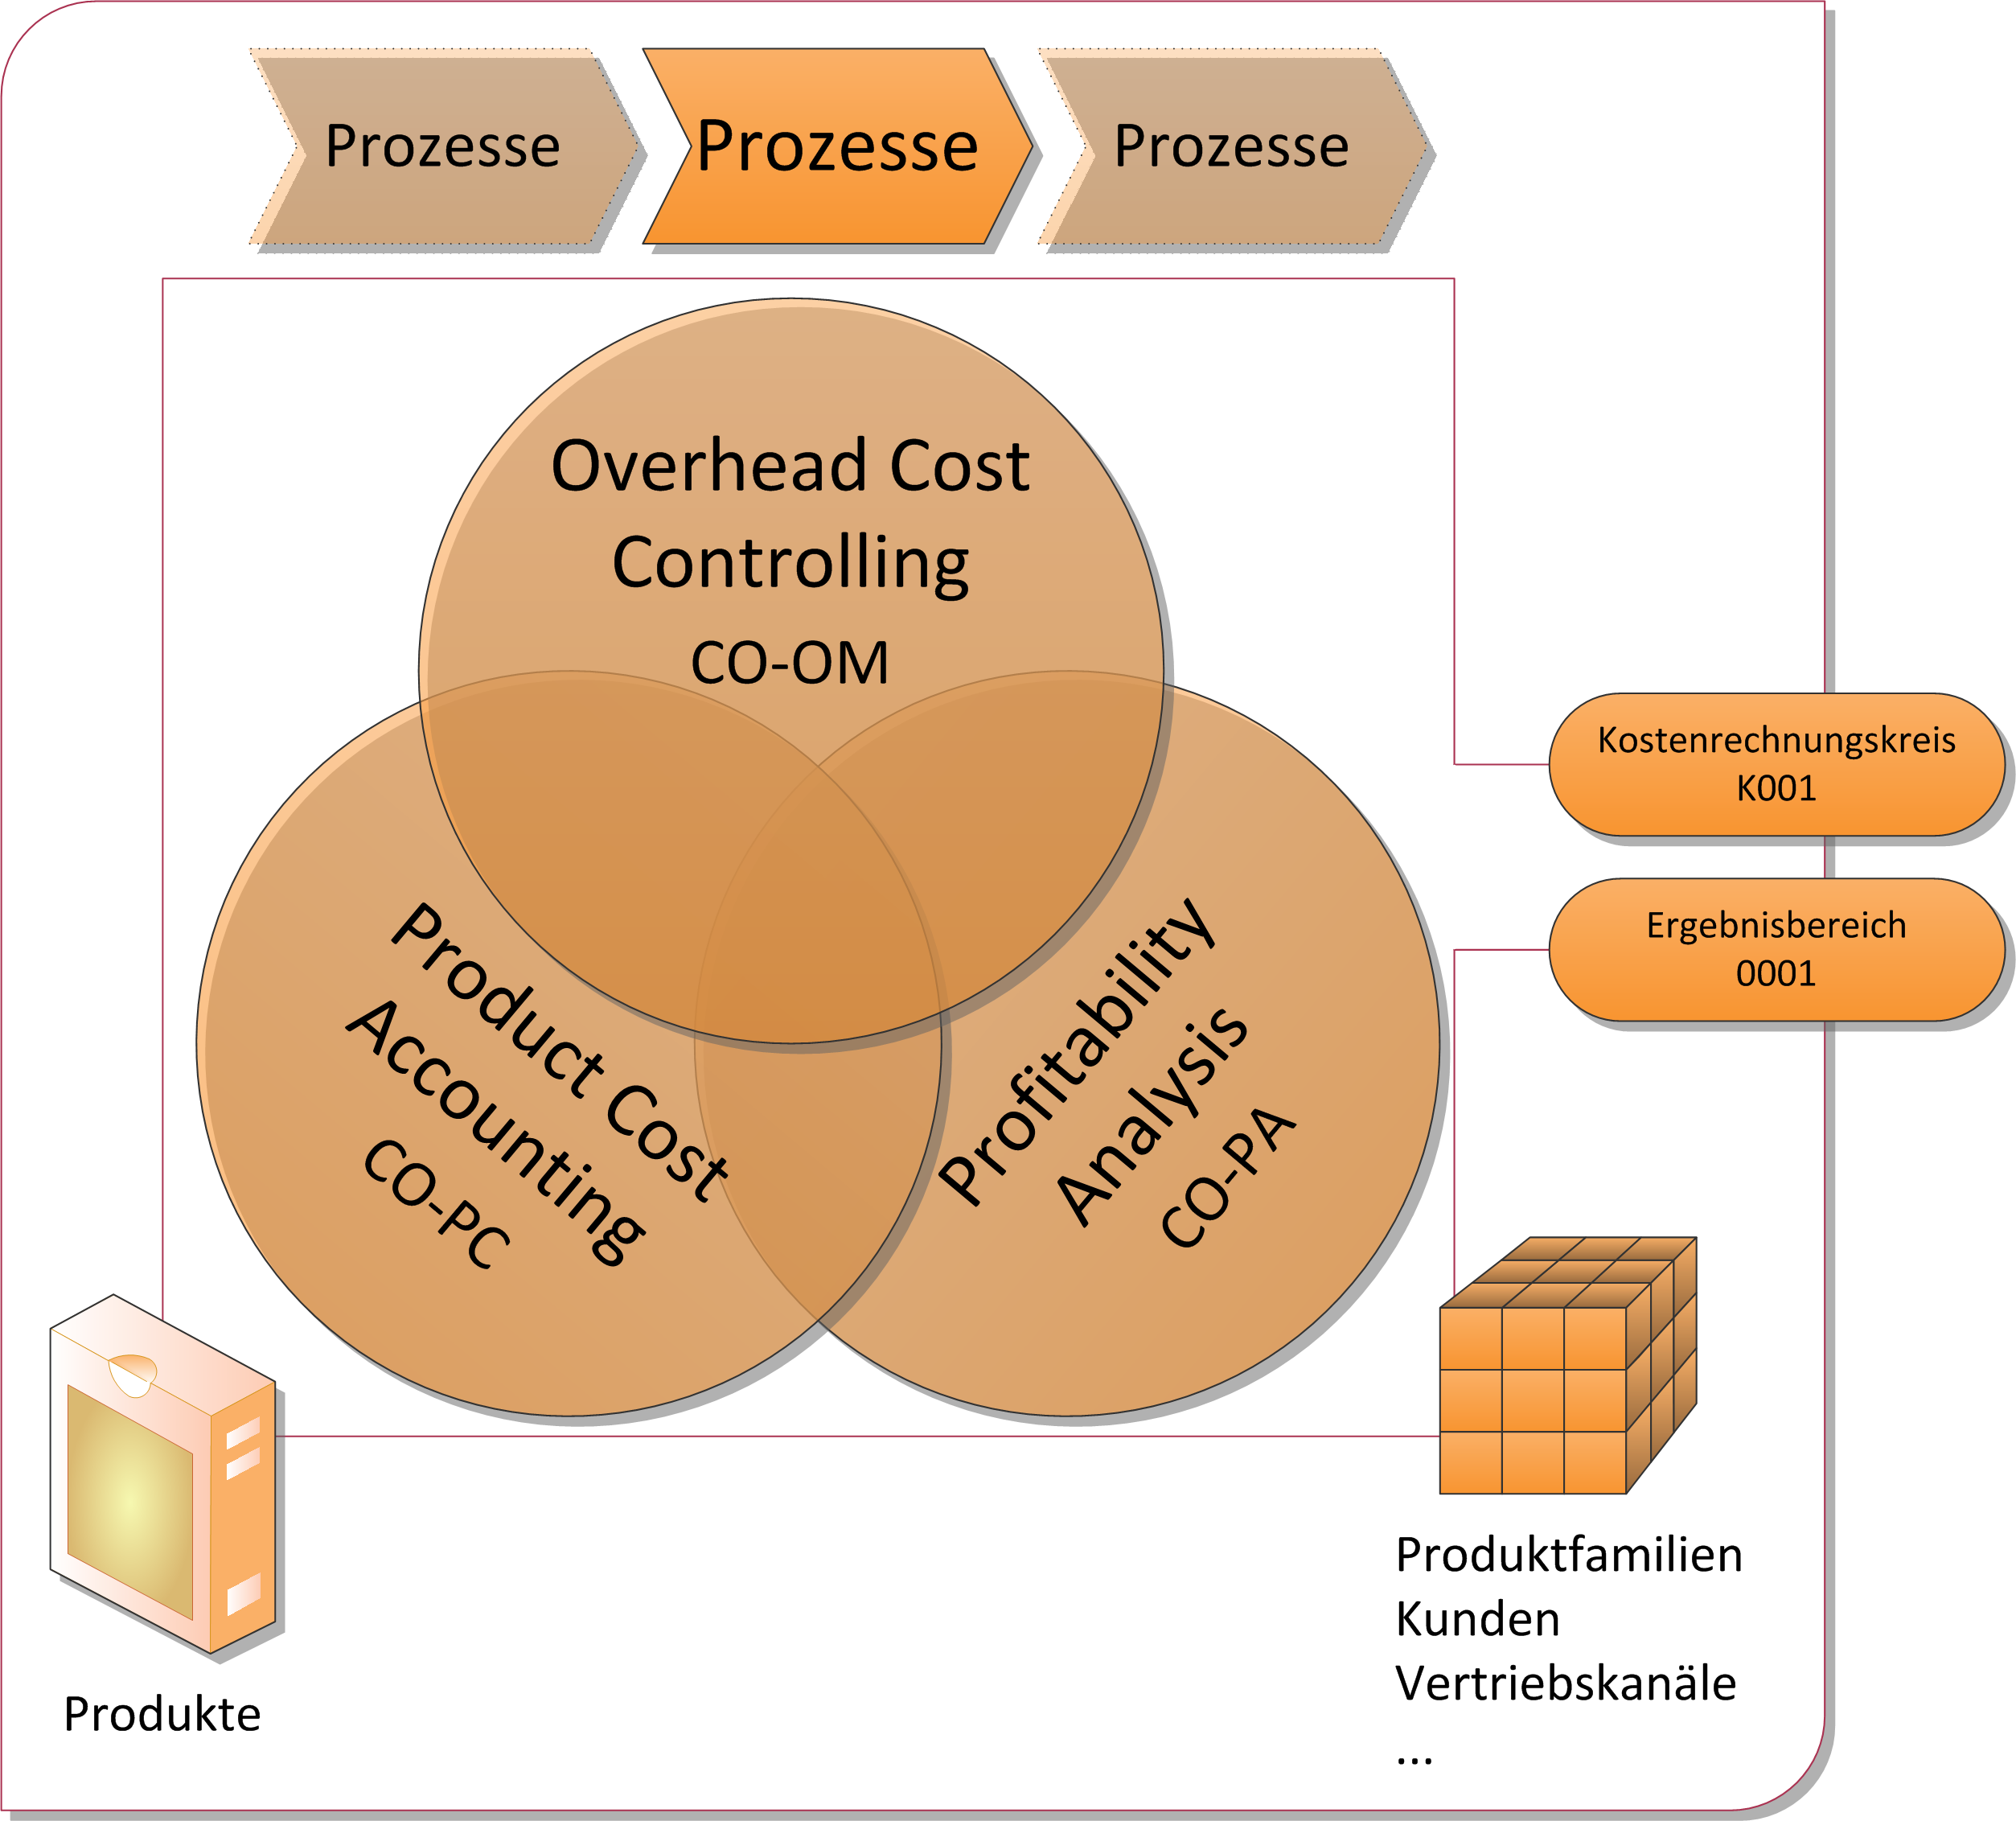
\includegraphics[width=0.8\textwidth]{Images/managementAccounting.png}

   {\footnotesize In Anlehnung an: \cite{SAPCOOMABC2001}, S. 11}
   \caption[Management Accounting -- Die Komponente CO]{Management Accounting -- Die Komponente CO}\label{abb3}
\end{center}
\end{figure}\noindent
\\Die zentrale Organisations- und Kontierungseinheit im Controlling ist der Kostenrechnungskreis (Vgl. s. Abb. \ref{abb4}, S. \pageref{abb4}). Mithilfe des Kostenrechnungskreises können Sie Ihr Unternehmen im Hinblick auf die Kostenrechnung im SAP-System buchungskreisübergreifend struktuieren\footnote{Vgl. \cite{Patel2009}, S. 291}\footnote{Vgl. \cite{Friedl2008}, S. 23}\footnote{Vgl. \cite{Klein2010}, S. 99}. SAP ERP stellt verschiedenen Kostenträger zur Verfügung, um alle anfallenden Kosten und Erlöse im Unternehmen zu strukturieren und möglichst exakt darstellen zu können. Der Begriff Kostenträger bzw. Kostensammler beschreibt Objekte wie Kostenstellen, Kostenarten und Innenaufträge\footnote{Vgl. \cite{Patel2009}, S. 208}. 
\subsubsection{Overhead Cost Controlling}
\begin{floatingfigure}[htbpr]{0.5\textwidth} 
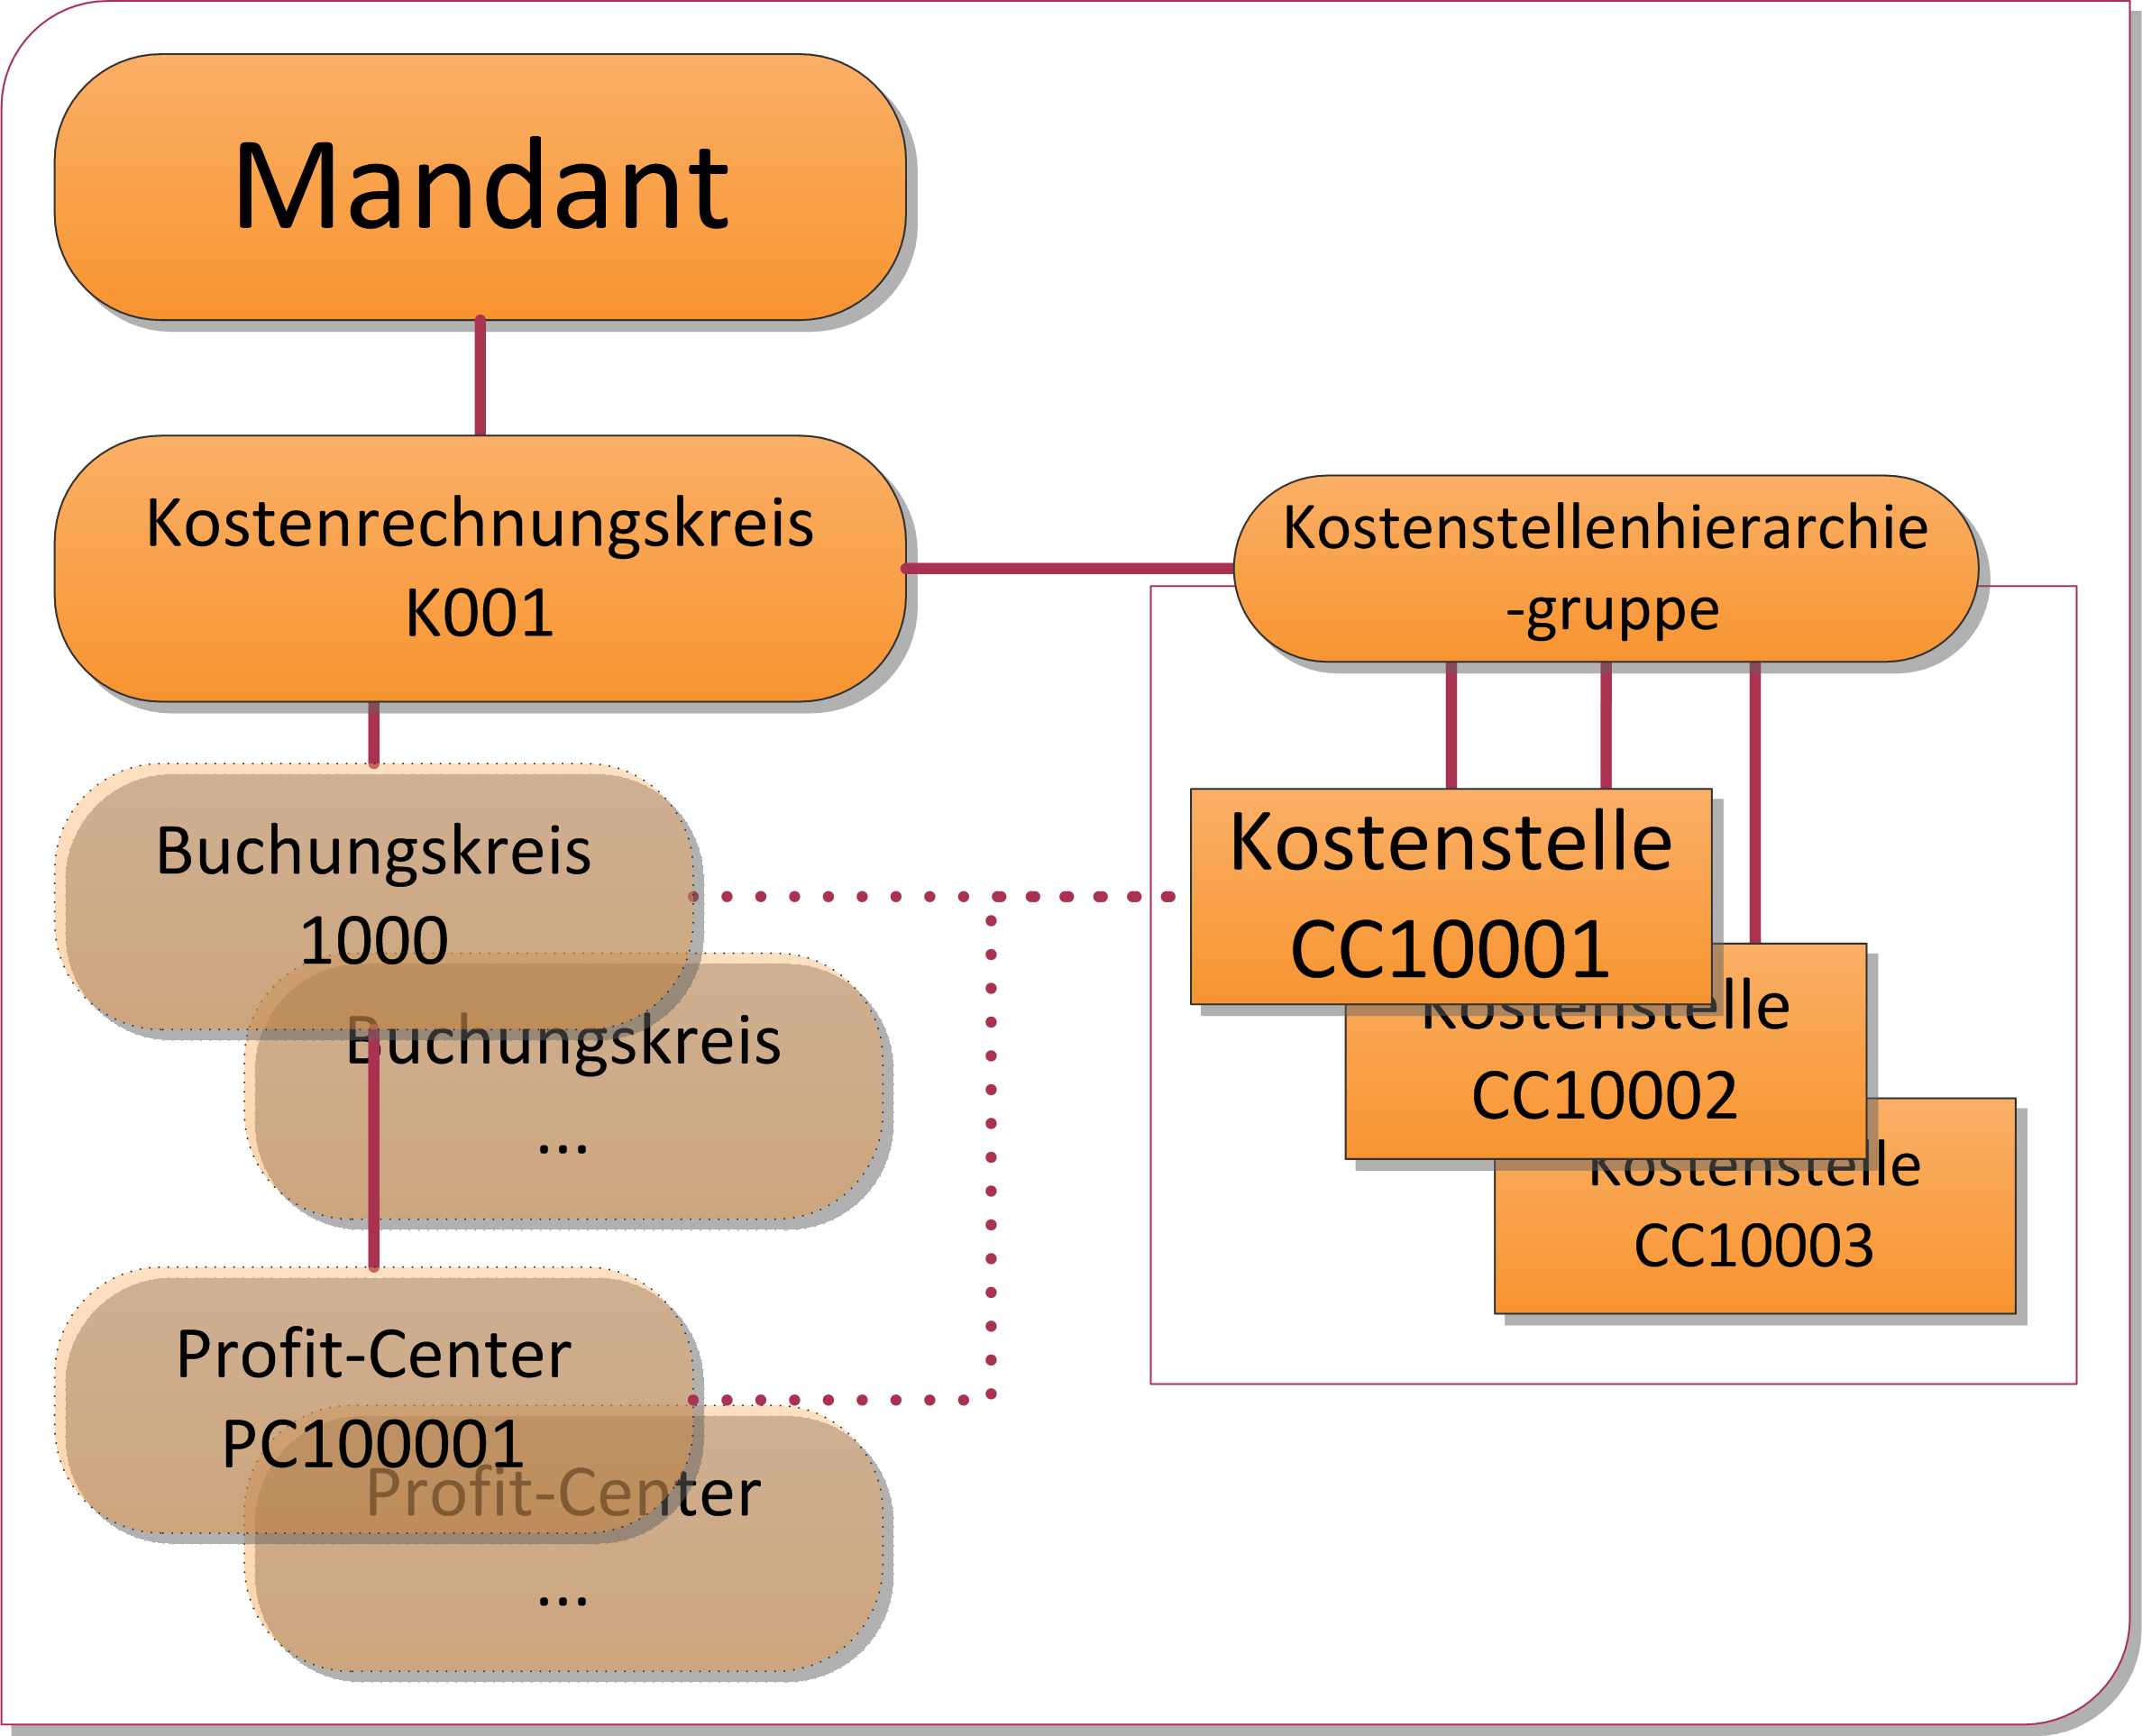
\includegraphics[width=0.5\textwidth]{Images/kostenRechnungskreis.png}
\begin{flushright}
   %{\footnotesize In Anlehnung an: \cite{Hefner2001}, S. 100}
   \caption[Kostenrechnungskreis in SAP ERP Financials]{Kostenrechnungskreis in \\SAP ERP Financials}\label{abb4}
\end{flushright}
\end{floatingfigure}\noindent
\abk{Cost Center Accounting}{dt. Kostenstellenrechnung (SAP CO-OM-CCA)}
\abk{Internal Order Accounting}{dt. Innenaufträge (SAP CO-OM-OPA)}
\abk{Profit Center Accounting}{Profit-Center Rechnung (EC-PCA)}
\abk{Overhead Cost Controlling}{dt. Gemeinkostenrechnung}
Overhead Cost Controlling (dt. Gemeinkostenrechnung) ist vor allem den Gemeinkosten gewidmet. Als Gemeinkosten\footnote{Personalkosten, Anlagekosten, Reisekosten, Beschaffungskosten, usw.} werden in der Regel Kosten bezeichnet, die im Gegensatz zu den direkten Kosten, nicht direkt den Produkten oder Dienstleistungen zugeordnet werden können. SAP ERP Financials unterstützt überwiegend mit der Kostenstellenrechnung, Innenauftragsrechnung und Prozesskostenrechnung die genaue Aufzeichnung, Analyse, Verrechnung und Buchung von Gemeinkosten\footnote{Vgl. \cite{Patel2009}, S. 288}\footnote{Vgl. \cite{SAPCOOMCCA2001}, S. 18}. 

Als Fundament des Controllings in SAP gilt die Kostenstellenrechnung\footnote{Vgl. \cite{Klein2010}, S. 98}.
Die Kostenstellen in SAP werden unterhalb eines Kostenrechnungskreises in einer Kostenstellenhierarchie organisiert und entsprechen in der Regel der Struktur eines Unternehmens im Hinblick auf Büros, Abteilungen, Bereiche und Standorte. Der Kostenstellenverantwortliche wird in den Stammdaten der Kostenstellen hinterlegt und verantwortet sowohl die präzise Aufzeichnung und Abrechnung von Kosten in ihren Kostenstellen, sowie die Einhaltung des vorgesehenen Budgets. Die Integration, z. B. die automatische Kostenstellenfindung in anderen SAP Komponenten, wird durch eine Zuordnung der Organisationseinheiten wie einem Buchungskreis oder einem Profit-Center ermöglicht\footnote{Vgl. \cite{Patel2009}, S. 296 f.}.
Mithilfe der Kostenstellenrechnung wird im SAP-System eine präzise Kostenplanung, -erfassung und -aggregation vorgenommen. Es erfolgt eine Zuordnung der Gemeinkosten nach ihren Kostenarten\footnote{Vgl. \cite{SAPOMCEL2001}, S. 6} auf die Kostenstellen und im Rahmen der innerbetrieblichen Leistungsverrechnung können Kosten der Vorkostenstellen auf die Endkostenstellen weiterverrechnet werden\footnote{Vgl. \cite{Friedl2008}, S. 24}. Außerdem wird eine Rückverfolgung der Kosten von den zugewiesenen Werten bis zu deren Ursprung ermöglicht. 
Auf diese Weise ist die Transparenz und Kontrolle der operativen Verfahren sichergestellt\footnote{Vgl. \cite{Patel2009}, S. 288}. 
Die Kostenstellenrechnung gibt an, wo im Unternehmen welche Kosten angefallen sind\footnote{Vgl. \cite{Friedl2008}, S. 24}.

Innenaufträge stellen eine weitere Möglichkeit zur Ermittlung der Istkosten einer internen Initiative, eines internen Jobs oder eines einfachen Projekts dar\footnote{Vgl. \cite{Patel2009}, S. 289}. Als klassisches Beispiel veranstaltet die Marketingabteilung einen Messeauftritt. Die anfallenden Kosten werden als Messekosten mit der Kostenstelle des Marketings verrechnet. In der Kostenstellenrechnung können nun Rückschlüsse auf die Kostenart und den Ursprung der Kosten gezogen werden. Wird für diesen Messeauftritt ein Innenauftrag erstellt, können die Kosten in Art und Ursprung diesem speziellen Vorgang zugeordnet und noch differenzierter betrachtet werden. Neben den Kosten können auch Messeerlöse auf den Innenauftrag verrechnet und ihnen gegenüber gestellt werden\footnote{Vgl. \cite{Klein2010}, S. 184 f.}. 
So bieten Innenaufträge im Vergleich zu Kostenstellen eine höhere Transparenz, da die Kostenanalyse für einzelne Jobs und nicht für die gesamte Kostenstelle durchgeführt wird. Innenaufträge können während des vollständigen Lebenszyklus eines Jobs überwacht werden, indem fortlaufend ein Vergleich der Istkosten und -erlöse mit den Plankosten und -erlösen stattfindet. Die für Innenaufträge anfallenden Kosten können an weitere Innenaufträge, Kostenstellen usw. weiterberechnet werden\footnote{Vgl. \cite{Patel2009}, S. 289}.

Die Geschäftsprozessplanung ist ein Vorgang, der in nahezu jedem Unternehmen anders gehandhabt wird. Branchenspezifische Besonderheiten, besondere organisatorische Strukturen und Verantwortlichkeiten erzwingen eine firmenindividuelle Gestaltung der Prozesse\footnote{Vgl. \cite{Friedl2008}, S. 24}. Einen Einblick in die Rentabilität dieser Geschäftsprozesse erlauben die zahlreichen Techniken und Methoden der Prozesskostenrechnung (CO-OM-ABC, Activity-Based Costing)\abk{Activity-Based Costing}{CO-OM-ABC, Prozesskostenrechnung}. Die Prozesskostenrechnung ermöglicht es, die Istkosten von Geschäfts-prozessen, Produkten und Dienstleistungen transparent zu gestalten. Im Gegensatz zur verantwortungs- und funktionsorientierten Kostenstellenrechnung bildet sie eine vorgangsorientierte und funktionsübergreifende Sicht der Abläufe in Unternehmen ab. Dadurch ergänzt die Prozeßkostenrechnung die Kostenstellenrechnung\footnote{Vgl. \cite{SAPCOOMABC2001}, S. 11}. 
Um Betriebskosten \\präziser zu bestimmen, kann die Prozesskostenrechnung mit den operativen und logistischen Komponenten des SAP-Systems (z. B. Logistik) integriert werden. Parameter wie z. B. der Anzahl an Kreditorenrechnungen, Bestellungen oder abgewickelte Kundenbesuche werden dann zur Berechnung hinzu gezogen\footnote{Vgl. \cite{Patel2009}, S. 289}. 
Die Istkosten für Geschäftsprozesse, Produkte und Dienstleistungen werden transparent darstellt und verbessert die Produktkalkulation\footnote{Vgl. \cite{Patel2009}, S. 318 f.}.


\subsubsection{Product Cost Accounting}
\abk{Product Cost Controlling}{dt. Produktkosten-Controlling (CO-PC)}
Unabhängig von der Branche bielcl jedes Unicmehmen ein Produkt
oder eine Dienslleisiung an. Die Konirolle über die Produkikoslen ist
lur jede Untemehmensan ein wesemlicher Aspeki der Winschatlich-keil.
Die SAP-Komponente Produkt-kostencontrolling stellt ein präzises, detailliertes, transparentes und le-xibles Framework zur Kalkulation und Erfassung der Produkt- und
Dienstleistungskosten eines Unternehmens bereit. Das Werkzeug für das Produktkostencontrolling verliigi z. B. über
Funktionen zur Senkung der direkten oder indirekten Fenigungskos-ten. zur Kostenschätzung für eine potenzielle neue Produktlinie oder
zur Kostenkalkulation von Änderungen an vorhandenen Produkten\footnote{Vgl. \cite{Patel2009}, S. 355}.
Das SAP Projektsystein kann für alle Gemeinkosten-, Invesiilions- oder
Fenigungsprojekte verwendet werden. 
Der lexible Projekiemwurf und die Integration mit den SAP-Buch-haliungs- und -Logistikkomponenten ermöglichen Ihnen eine voll-ständige Kontrolle über die Art und Zielsetzung eines Projekts im
SAP Projektsystem.
> Die Imegralion mit anderen SAP-Komponenicn ermöglicht Ihnen
die Inilüerung, Verwaltung und Durchfuhrung von End-to-End-GeschäfisVorgängen - vom Kundenangeboi bis zur abschließenden
Lieferung - (Qr Kundenprojekie (z. B. Kundeneinzelfenigung).
> Die präzise Kostenplanung und -Überwachung hinsichtlich des Bud-gets lässt Projekt Vorgänge transparent erscheinen und ermöglicht es
Ihnen. Problemen schon zu einem frühen Zeitpunkt entgegenzuwir-ken.
> Die Verfügbarkeit von Fakturierungsfunktionen. wie beispielsweise
Faktuierungspläne und aufwandsbezogene Fakturierung, sowie die
vollständige Integration mit dem Vertrieb erleichten Ihnen eine
frühzeitige Planung von Projektcrlösen. sodass Sie sich einen Über-blick über einen möglichen Gewinn oder Verlust verschaffen kön-nen.
> Das Projckt-Cash-Management ermöglicht Ihnen eine Bewertung
und Überwachung der Kapitalbildung in Projekten, sodass Sic pro-aklive Maßnahmen bei der Verwaltung des Projckt-Cashlows
ergreifen können.
> Sie können den technischen sowie den winschaftlichen Fortschritt
von Projekten mithilfe zahlreicher Standardbeichte oder gemäß
Ihren Anforderungen erstellten Berichten überwachen, analysieren
und bewerten\footnote{Vgl. \cite{Patel2009}, S. 253 f.}.
Materialkosten
 Fertigungskosten
 Gemeinkosten
 Herstellkosten
. Vertrieb \& Verw- 
= Selbstkosten

Das Produktkostencontrolling bietet umfassende Unterstützung für
verschiedene Fertigungsumgebungen, wie Lagerfertigung, Einzel-fertigung, Seienfertigung usw.
> Mit der Produktkostenplanung können Sie Mateialkosten und Pro-duktkosten planen, um Ihre Kostenstruktur einschließlich der Ferti-gungskosten, Gemeinkosten, Materialkosten und Leistungskosten
analysieren zu können.
> Das Maierial-Ledger umerstülzt Sie bei der Durchführung von Ist-kalkulationen zur Bewertung Ihres Bestands unter Berücksichtigung
unvermeidbarer Preisdifferenzen, und es ermöglicht Ihnen eine
Bestandsführung mit mehreren Währungen oder Bewenungen.
> Eine einfache Berechnung der Plankosten wird durch das Easy Cost
Flanning gewährt. Auf Grundlage der Kalkulationsergebnisse wer-den Bestellanforderungen, Bestellungen, Wareneingänge und
andere relevante Vorgänge automatisch ausgelöst.
Sie haben Zugiff auf zahlreiche deiailliene Berichie, die über ver-schiedene Informaiionssysteme. unier anderem iur das Produktkos-tencontrolling, für das Material-Ledger und für Mischkalkulationen
erstellt wurden\footnote{Vgl. \cite{Patel2009}, S. 392 f.}



\subsubsection{Profitability Analysis} %CO-PA
\abk{Profitability Analysis}{dt. Ergebnis- und Marktsegmentrechnung (SAP CO-PA)}
Mit dem Verschwinden geograflscher und wirtschafilicher Grenzen
sind auch die Märkte für Unternehmen gewachsen. Dieser Umstand
schafft neben Chancen allerdings auch Herausforderungen, z. B. einen
weltweiten Wettbewerb, unterschiedliche Kundenwünsche und eine
steigende Anzahl an Faktoren, die die Gewinnmargen direkt und
indirekt beeinflussen. Um einen Wettbewerbsvortei! zu erlangen und
neue Strategien festlegen zu können, müssen Sie ermitteln können,
wie sich Ihre einzelnen Produkte und Dienstleistungen in den unter-schiedlichen Marktsegmenten behaupten. Des Weiteren benötigen Sie
aktuelle, nach Kunden und Produkten aufgeschlüsselte Vertriebs Infor-mationen. Die Ergebnis- und Marktsegmentrechnung. auch schlicht Ergebnis-rechnung genannt, (engl. Controlling - Profitabilily Analysis) in SAP
ERP Financials bietet Ihnen alle nötigen Funktionen für ein anforde-rungsgerechtes Reporting in diesem Bereich, z.B. für eine Deckungs-beitragsrechnung. Sie können für verschiedene Marktsegmente
Absatzzahlen. Umsätze. Kosten des Umsatzes. Vertriebskosten, Mar-gen etc. planen sowie Daten zu Geschäftsvorgängen aus anderen SAP-Komponenten erfassen und verteilen. Außerdem bietet die SAP-Ergeb-nisrechnung umfassende Reponingmöglichkeiten und erweiterte Ana-lysefunktionen. Durch den Einsatz des Informationssystems können Sie die in
Geschäftsvorgängen mit Planwerten gesammelte Daten analysieren
und einen detaillierten Vergleich der für Ihr Unternehmen wichtigen
Rentabililätskriterien durchführen.Wenn Sie über einen Einsatz von SAP ERP Financials nachdenken,
müssen Sie entscheiden, ob Sie die Ergebnisrechnung mit oder ohne
Proßt-Center-Rechnung verwenden möchten. Die Profit-Center-Rech-nung bietet Ihnen eine eingeschränkte Funktion für die Reniabilitäts-analyse, die allerdings relativ einfach umzusetzen ist. Die Ergebnis-rechnung baut bei der Bereitstellung präziser Daten auch auf anderen
SAP-Komponenten, insbesondere auf den Venieb auf. Wenn diese
anderen SAP-Komponenten noch nicht in vollem Umfang genutzt wer-den, können Sie das Potenzial der Ergebnisrechnung unter Umständen
nicht voll ausschöpfen. \footnote{Vgl. \cite{Patel2009}, S. 395 ff.}. 
Die ProfU-Center-Rechnung bietet eine vereinfachte Umgebung zur
Berechnung der Rentabilität einzelner Untemehmensbereiche.
> Mit der Ergebnisrechnung können Sie die Rentabilität nach Produkt,
Markt. Kunde, Spane und anderen Kiteien anhand von Finanzkon-ten und lexiblen, kundenspeziischen Werten analysieren.
> Über die leistungsstarke Integration können Sie Daten aus anderen
SAP-Komponenten, wie z. B. Finanzbuchhaltung, Vertieb. Mateial-wirtschaft. Gemeinkostencontrolling und Produktkostencontrolling
usw., sammeln. 
Mithilfe des umfangreichen Planungseinstiegs können Sie den
Absatz, Erlös und die Rentabilität für verschiedene Ergebnisobjekte
planen und den gesamten Planungsprozess beziehungsweise Teile
davon aus unterschiedlichen Perspektiven betrachten.
> Anhand der austuhrlichcn Berichte können Sic den Deckungsbei-trag, Marktsegment- und Kalkulalionsvergleiche usw. nach verschie-denen Merkmalen (z. B. Kunden, Produkte) oder Merkmalshierar-chien analysieren\footnote{Vgl. \cite{Patel2009}, S. 428 f.}.



























%############ ALTE ARBEIT!! ### ALS COPY/PASTE VORLAGE ###################
%\label{sec:spc}
%In diesem Kapitel werden die wesentlichen Aufgaben des Projektcontrollings im strategischen Projektmanagement erklärt. \\
%Neben der strategischen Projektplanung und Vorgehensweise bei der Projektauswahl, wird ein besonderer Schwerpunkt auf die Managementmethode der Projekt-Scorecard zur Priorisierung und Steuerung von Projekten gelegt. Den Abschluss bilden Betrachtungen zur strategischen Kontrolle.
%\subsection{Strategisches Projektmanagement}
%Christian Kunz kommt zur Erkenntnis, dass in der Literatur die Bedeutung von Projekten zur Implementierung von Unternehmensstrategien weitgehend akzeptiert ist. Weiterhin bestünde Einigkeit, dass aufgrund der Vielzahl der Projekte zur Implementierung von Strategien sowie der inhaltlichen Verknüpfung dieser untereinander eine Führungsfunktion die Abstimmung und Kontrolle der Projektgesamtheit übernehmen sollte. Das strategische Projektmanagement entspricht somit einer Führungsfunktion und kann als strategisch bedeutend eingestuft werden\footnote{Vgl. \cite{Kunz2007}, S.~11}.
%Für die Effektivität und Effizienz eines projektorientierten strategischen 
%Management ist ein leistungsfähiges strategisches Projektcontrolling eine wesentliche Voraussetzung\footnote{Vgl. \cite{Foschiani1999}, S.~133}.
%Weiterhin ist das strategische Projektmanagement vom Programm-Management sowohl inhaltlich als auch begrifflich abzugrenzen. Programm-Management orientiert sich an einer zeitlich befristeten Anordnung vieler Teilprojekte, die insgesamt ein Großprojekt darstellen und mit Ergebnisverantwortung verbunden sind. Nach Beendigung des Programms wird auch die temporäre Struktur des Programm-Managements abgebaut. Demgegenüber stellt das strategische Projektmanagement eine dauerhafte Steuerungseinrichtung im Unternehmen dar, die eng mit dem restlichen Führungssystem des Unternehmens verbunden ist. Wie in Abbildung ersichtlich wird, besteht ein Projektportfolio somit sowohl aus Einzelprojekten als auch aus Projekten, die Bestandteil eines Programms sind\footnote{Vgl. \cite{Kunz2007}, S.~21}.
%\begin{figure}[htbp]
%%\begin{floatingfigure}[htbpr]{0.43\textwidth} 
%\begin{center}
%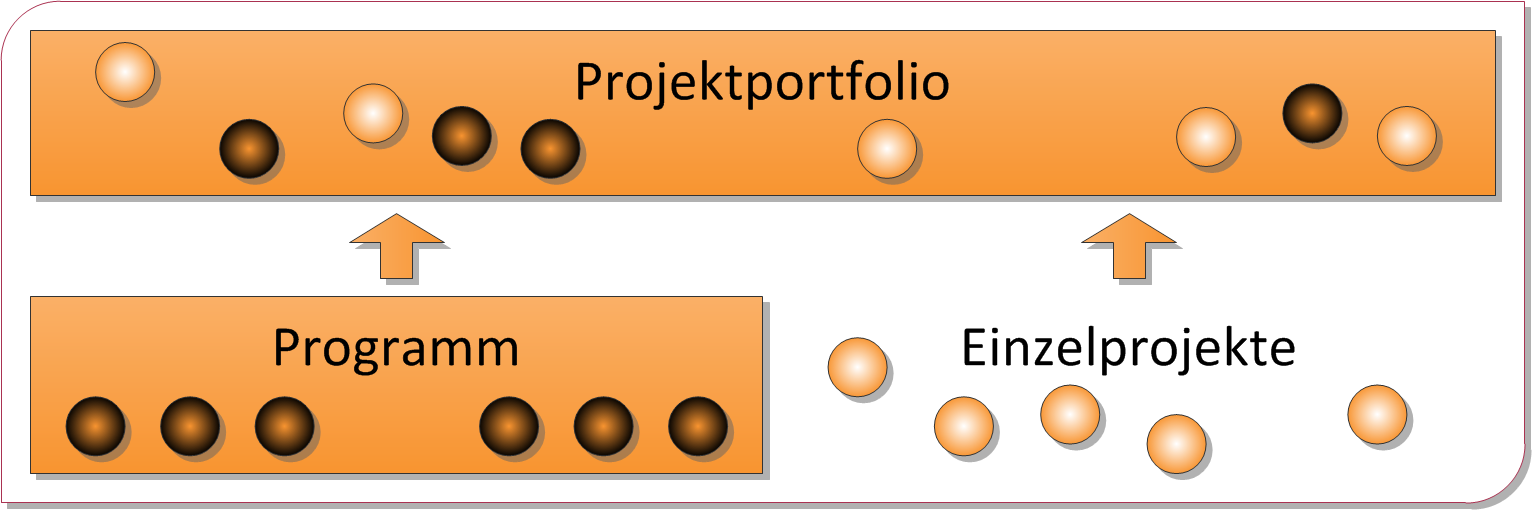
\includegraphics[width=0.8\textwidth]{Images/projektportfolio.png}
%\label{abb5}
%
%   {\footnotesize In Anlehnung an: \cite{Foschiani1999}, S.21--22]}
%   \caption[Zusammenhang von Einzelprojekten, Programm und Projektportfolio]{Zusammenhang von Einzelprojekten, Programm und Projektportfolio}
%\end{center}
%
%
%
%
%\end{figure}
%%\end{floatingfigure}
%
%\subsection{Strategische Projektplanung}
%\label{sec:SPP}
%Grundlage der strategischen Projektplanung sind die Unternehmensziele, die wesentliche Auswahlkriterien für die Projekte liefern. Die Projekte müssen mit den strategischen Zielen harmonieren. Ein Unternehmen mit dem strategischen Ziel schnelles Wachstum durch Ausweitung des Marktanteils wird Projekte anders beurteilen als ein Unternehmen, das die Gewinnmaximierung durch Kostensenkung verfolgt.
%Aufgrund der hohen Projektanzahl im Projektportfolio des strategisches Projektmanagements konkurrieren unterschiedliche Projekte um zumeist knappe Unternehmensressourcen\footnote{Vgl. \cite{Kunz2007}, S.~1}. Die Projektwünsche erreichen das Portfolio entweder Top-Down durch die Unternehmensleitung oder Bottom-Up durch die Fachbereiche. Dabei ist sicherzustellen, dass Projektideen nicht von vornherein abgeblockt oder bevorzugt werden. Jeder Vorschlag sollte zunächst die gleiche Chance haben. Ansonsten besteht die Gefahr, dass sinnvolle Vorhaben nicht realisiert werden\footnote{Vgl. \cite{Fiedler2008}, S~36}.
%Zu Beginn der Projektportfolioplanung ist eine Gesamtbetrachtung aller Projekte anzustreben. Deswegen sollte man auch die bereits genehmigten und die laufenden Projekte in die Analyse einbeziehen. Es kann durchaus sein, dass schon genehmigte Vorhaben aufgrund der nachfolgenden Bewertung verschoben oder nicht realisiert werden\footnote{Vgl. \cite{Fiedler2008}, S.~39}.
%\begin{figure}[htbp]
%%\begin{floatingfigure}[htbpr]{0.43\textwidth} 
%\begin{center}
%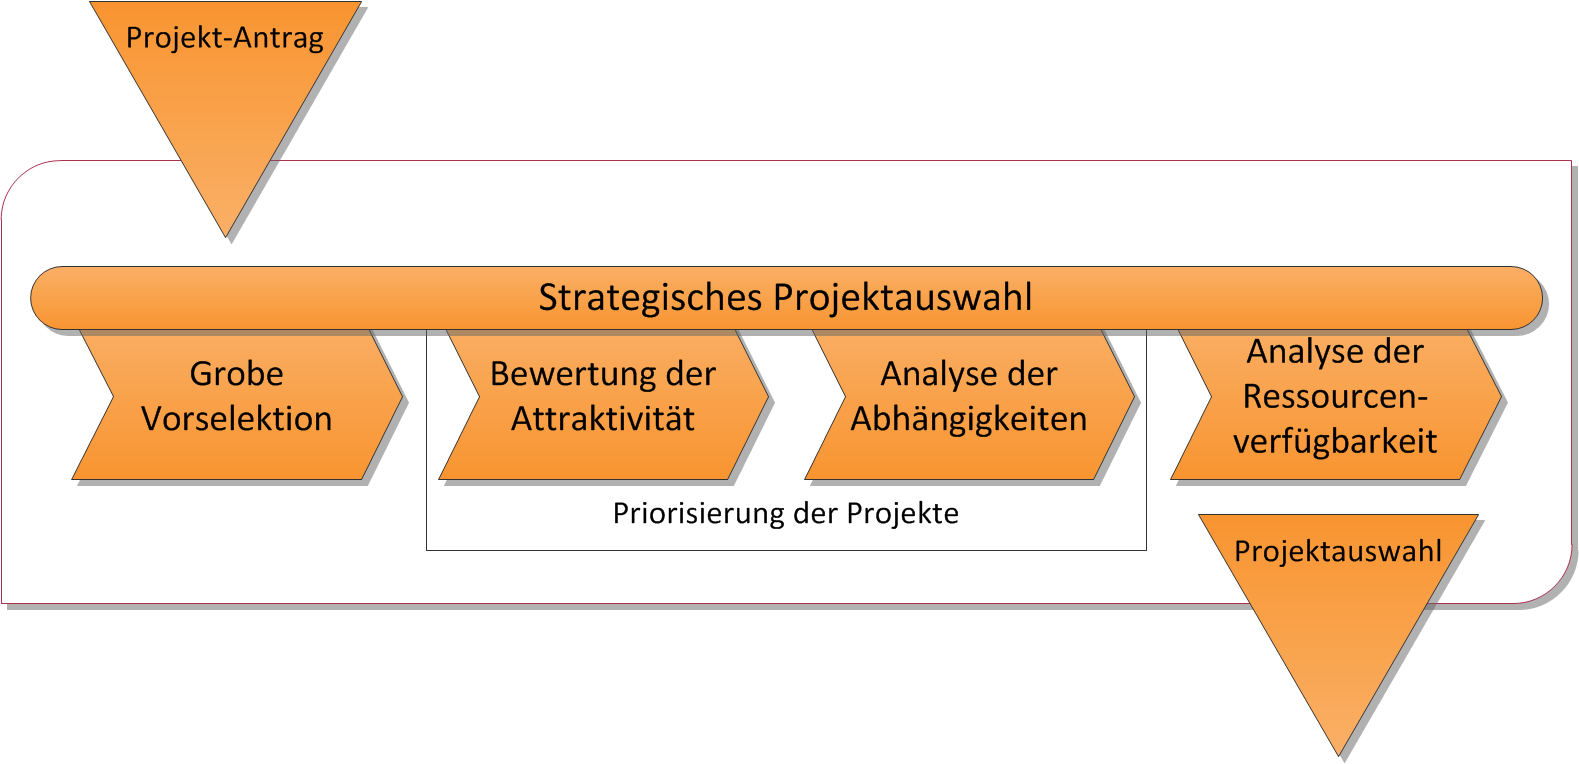
\includegraphics[width=0.8\textwidth]{Images/prozessProjektauswahl.png}
%\label{abb6}
%
%   {\footnotesize In Anlehnung an: \cite{Archer1999}, S. 208}
%   \caption[Prozess der strategischen Projektauswahl]{Prozess der strategischen Projektauswahl}
%\end{center}
%
%\end{figure}
%%\end{floatingfigure}
%In der Abbildung \ref{abb6} auf Seite \pageref{abb6} wird der Prozess der strategischen Projektauswahl dargestellt. Die strategische Projektplanung nutzt diesen Ablauf, um die vorgeschlagenen Projekte im Einklang mit der Unternehmensstrategie auf die wirklich wichtigen zu beschränken. Die hierbei zum Einsatz kommenden Methoden liefern einheitliche Beurteilungskriterien und reduzieren die Gefahr, knappe Ressourcen zu verschwenden. Die strategische Projektplanung liefert so eine  Entscheidungsfundierung, auf Basis derer das Management die letztendliche Projektauswahl trifft\footnote{Vgl. \cite{Fiedler2008}, S.~85}.
%
%Die grobe Vorselektion prüft neben der Machbarkeit, ob die Projektvorschläge den strategischen Zielen offensichtlich widersprechen. In dieser Phase kann es zur Definition von Muss-Projekten kommen. Dabei handelt es sich um Vorhaben, die z. B. aufgrund gesetzlicher Vorschriften unumgänglich sind\footnote{Vgl. \cite{Fiedler2008}, S.~41}.
%
%Im Schritt Bewertung der Attraktivität wird die Attraktivität der Projekte für das unternehmen detailliert bewertet. Die wichtigsten Bewertungskriterien sind:
%\begin{compactitem}
%\item Strategische Bedeutung (Wettbewerbsvorteile, Kundenorientierung),
%\item Dringlichkeit,
%\item Wirtschaftlichkeit,
%\item Risiko,
%\item Kosten (Entwicklungskosten, Folgekosten),
%\item Ressourcenbedarf\footnote{Vgl. \cite{Fiedler2008}, S.~41}.
%\end{compactitem}
%Rudolf Fiedler schreibt über die Aufgabe des Projektcontrollings bei der Bewertung der Attraktivität:
%\begin{quote}
%Das Projektcontrolling hat die Aufgabe, Hilfestellung beim Einsatz von Bewertungsinstrumenten zu geben und die Konsistenz der zur Beurteilung herangezogenen Daten zu prüfen.\footnote{\cite{Fiedler2008}, S. 42}
%\end{quote}
%Für eine Gesamtbetrachtung aller Einflussfaktoren der Projektbewertung bietet sich die Nutzwertanalyse an. Weitere Instrumente zur Bestimmung der Attraktivität sind auch Portfolios und Wirtschaftlichkeitsrechnungen. Ein weiterer wichtiger Bestandteil ist die Risikoanalyse, um das Erfolgspotenzial der Projekte abzuschätzen\footnote{Vgl. \cite{Fiedler2008}, S. 42}.
%[s. Kommentar] %zu wenig? dann noch Bilder von Nutzwert, Risiko, Portfolios und Wirtschaftlichkeitsanalysen einfügen.
%
%In der Analyse der Abhängigkeiten werden die gegenseitigen Einflüsse der Portfolioprojekte untersucht. Ein Projekt kann bereits in der Konzeptionsphase anderer Projekte zur veränderten Vorraussetzungen führen. Auch müssen manche Projekte mit anderen zusammen realisiert werden, da nur so das Gesamtziel erreicht werden kann. Gerade wenn verschiedene Projekte aufeinander aufbauen, hat dies ggf. signifikante Auswirkungen auf die Kosten der Umsetzungen.
%Die Ergebnisse der Auswirkungen stehen also in einem kausalen Zusammenhang mit der Attraktivität und bestimmen gleichermaßen die Priorität der Vorhaben\footnote{Vgl. \cite{Fiedler2008}, S. 79}. 
%
%Nachdem die Projekte vorselektiert, detailliert analysiert und priorisiert wurden, wartet die \glqq Hitliste\grqq der effektivsten Projekte aus die Zuteilung der meist knappen finanziellen Mittel und qualifizierten Ressourcen. Die Analyse der Ressourcenverfügbarkeit ordnet die erforderlichen Ressourcen nach Qualifikationsprofilen und die finanziellen Mittel nach den Budgets Projektklassen zu. Budgets für unterschiedliche Projektklassen werden gebildet, da gerade IT-Projekte oft große Teile des zur Verfügung stehenden Budgets aufzehren und so keine Mittel mehr für andere Projektarten zur verwendet werden können.
%Ergebnis dieser Untersuchung kann auch sein, dass Projektstarts verschoben, Leistungsumfänge gekürzt oder gar laufende Projekte gestoppt werden\footnote{Vgl. \cite{Fiedler2008}, S.~81--82}.
%
%\subsection{Strategische Projektkontrolle}
%\begin{figure}[htbp]
%%\begin{floatingfigure}[htbpr]{0.43\textwidth} 
%\begin{center}
%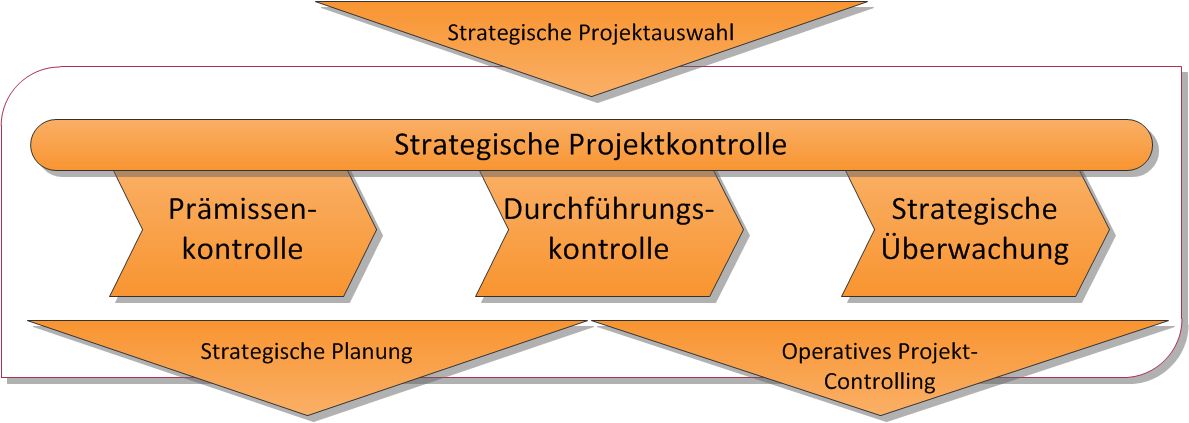
\includegraphics[width=0.8\textwidth]{Images/prozessStratKontrolle.png}
%   %{\footnotesize In Anlehnung an: \cite{Steinmann&Schreyogg2000}, S. 221}
%   \caption[Prozess der strategischen Projektkontrolle]{Prozess der strategischen Projektkontrolle}\label{abb6}
%\end{center}
%
%\end{figure}
%%\end{floatingfigure}
%Die strategische Projektkontrolle unterteilt sich in die drei wichtige Aufgaben\footnote{Vgl. \cite{Steinmann&Schreyogg2000}, S. 221}:
%\begin{compactitem}
%\item Prämissenkontrolle,
%\item Durchführungskontrolle und
%\item strategische Überwachung.
%\end{compactitem}
%Die Prämissenkontrolle untersucht während Projektauswahl und Projektdurchführung das gesamte Projektportfolio auf seine Ausgewogenheit und Stimmigkeit im Bezug auf die strategische Ausrichtung des Unternehmens. Sie stellt sicher, dass die in den Projektportfolios enthaltenen Projekte weiterhin den aktuellen strategischen Prämissen entsprechen. Hierzu sind gegebenenfalls einzelnen Projekte neu zu priorisieren\footnote{Vgl. \cite{Kunz2007}, S.~37}. 
%
%Im Rahmen der Durchführungskontrolle werden Informationen von allen Portfolioprojekten generiert, um den Fortschritt der einzelnen Projekte zu verfolgen. Mittels Definition messbarer Meilensteine, deren Ist-Ergebnisse mit der ursprünglichen Zielsetzung verglichen werden, werden strategisch relevante Problemfälle innerhalb des Projektportfolios identifiziert. Bei signifikanten Abweichungen sind Gegenmaßnahmen einzuleiten\footnote{Vgl. \cite{Kunz2007}, S.~37}~\footnote{Vgl. \cite{Fiedler2008}, S.~87}. Geeigneter Methoden der Durchführungskontrolle sind z. B. Variationen der Balanced Scorecard (Projekt--Scorecard), Checklisten oder Portfiliotechniken (Mapping Grids).
%
%Neben diesen Kontrollaktivitäten, die vor allem auf die Sicherstellung der zielgerichteten Durchführung von Projekten abzielen, fungiert die strategische Überwachung als ungerichtete flächendeckende Kontrolle als Ergänzung der beiden erstgenannten Kontrollen\footnote{Vgl. \cite{Fiedler2008}, S.~89}. Durch die Zusammenführung von Ergebniskontrolle und während der Projektdurchführung mitlaufender Wissensgenerierung werden die Projekte regelmäßig auf ihre Zielerreichung im Kontext der Unternehmensstrategien hin untersucht\footnote{Vgl. \cite{Kunz2007}, S.~37}.
%%\subsection{Projekt-Scorecard}
